\documentclass{beamer}

\usepackage[utf8]{inputenc}
\usepackage[german,vlined,boxed,ruled]{algorithm2e}

% Mathematische Erweiterungen der AMS
\usepackage{amssymb} 
\usepackage{amsfonts} 
\usepackage{amsmath}

%wird benoetigt um breite pdfs anzuzeigen
\usepackage{pgfpages} 
%\setbeameroption{show notes on second screen}
%\setbeameroption{show notes}

\usetheme{Goettingen}
\usecolortheme{default}
\usefonttheme{structuresmallcapsserif}
\useinnertheme{rectangles}
\setbeamertemplate{footline}[frame number]


\title{Approximative Algorithmen}
\subtitle{"Wie genau ist ungefähr?"}
\author[Robert B.]{Robert Bahmann}
\institute[HSRM]{Hochschule \textbf{RheinMain} University of Applied Sciences\\ Wiesbaden Rüsselsheim Geisenheim}

\begin{document}

\frame{\titlepage}
\section[Inhalt]{}
\frame{\tableofcontents}
\section{Einleitung}
\frame{
	\Large{Viele Probleme sind nicht effizient exakt lösbar solange $\mathbb P \not= \mathbb{NP}$}
	\note{Bekannte Beispiele dafür sind \textsc{Traveling Salesman Problem},\textsc{Knapsack} oder \textsc{List Schedule}}
}

\frame{
\frametitle{Approximationsalgorithmen}
\begin{block}{Warum Approximationsalgorithmen?}
	\begin{itemize}
		\item arbeiten in polynomieller Zeit
		\item<+-> produzieren Lösungen  mit \emph{garantierter} Güte
	\end{itemize}
\end{block}
}

\section{Grundlegende Eigenschaften}
\subsection{Güte/Performance}
\frame{
\frametitle{Güte/Performance}
\begin{block}{Güte/Performance}
	\begin{description}
		\item[Absolut] $\mathcal{AG}_{A}(\mathcal I)=|A(\mathcal I)-\text{OPT}(\mathcal I)|$
		\item[Relativ] $\mathcal{RG}_{A}(\mathcal I)=\text{max}\left\{
			\frac{A(\mathcal I)}{OPT(\mathcal I)},\frac{OPT(\mathcal I)}{A(\mathcal I)}
			\right\}$
	\end{description}
\end{block}
}
\subsection{Approximationsklassen}
\frame{
\frametitle{Approximationsklassen}
\begin{block}{APX}
	\textbf{A}\textbf{p}pro\textbf{x}imable - Gut approximierbare Probleme.
\end{block}
}

\frame{
\begin{block}{PTAS}
	\textbf{P}olynomial \textbf{T}ime \textbf{A}pproximation \textbf{S}cheme\\
	Beliebig gut Approximierbar auf Kosten des Fehlers.
\end{block}
}

\frame{
\begin{block}{FPTAS}
	\textbf{F}ully \textbf{P}olynomial \textbf{T}ime \textbf{A}pproximation \textbf{S}cheme\\
	Beliebig gut und schnell Approximierbar auf Kosten des Fehlers un der Laufzeit.
\end{block}
}

\section{Beispiel}
\frame{
	\frametitle{Job Scheduling}
		\begin{block}{\textsc{Job Scheduling}} Auf $p$ Prozessoren ($P_1,P_2,...,P_n$) sollen $t$ Tasks ($T_1,T_2,...,T_i$) verteilt werden. Dabei hat jeder Tasks eine Laufzeit $l_i$ die der Prozessor benötigt, um diesen abzuarbeiten.
		\end{block}
		%Ziel ist hier ganz klar die Laufzeit zu minimieren.
}
\frame{
	\frametitle{Job Scheduling - Beispiel}
	Auf einem Rechner mit einem Dual-Core müssen folgende Tasks abgearbeitet werden:\\
	\begin{center}
		\begin{tabular}
			{l|l} \textsc{Task}&\textsc{Zeit}\\
			\hline \hline 1 & 1\\
			\hline 2 & 2\\
			\hline 3 & 2\\
			\hline 4 & 4\\
			\hline 5 & 1\\
		\end{tabular}
	\end{center}
}

\frame{
	\frametitle{Job Scheduling - Beispiel}
	\begin{itemize}
		\item Core 1: $(0,P_1),(1,P_3),(3,P_2)$ 
		\item Core 2: $(0,P_4),(4,P_5)$
	\end{itemize}
	\begin{center}
		\begin{figure}[htbp]
			\centering	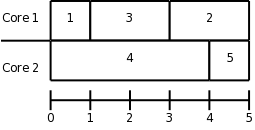
\includegraphics[height=50px]{../img/opt_prozessor_belegung.png}
		\end{figure}
		
	\end{center}
}

\subsection{JS Algorithmus}
\frame{
\frametitle{Job Scheduling - Algorithmus}
\begin{algorithm}[H]
\KwIn{$p$ Prozessoren,$t$ Taks und die Laufzeiten $l_i$ für jeden Task}
\KwOut{Eine Prozessorbelegung $S$ mit minimalen Makespan}
\caption{\textsc{Job Schedule}}
$S$ = null \;
\For{i = 1 to $m$}
	{$a_i$ = null\;}
\For{k = 1 to $n$}{
	Berechne das kleinste $i$ mit $a_i = min\{a_j;j \in \{1...,m\}\}$\;
	$S_k = a_i$\;
	$a_i = a_i + p_k$\;
	$S = S \cup \{(S_k,M_i)\}\;$}
return $S$\;
\end{algorithm}
}

\frame{
	\frametitle{Job Scheduling - Ausgabe}
	\begin{block}{Algorithmusausgabe}
	\begin{itemize}
		\item Core 1: $(0,P_1),(1,P_3),(4,P_5)$ 
		\item Core 2: $(0,P_2),(2,P_4)$
	\end{itemize}
	\end{block}
	\pause
	\begin{center}
		\begin{figure}[htbp]
			\centering	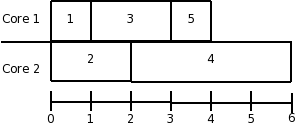
\includegraphics[height=50px]{../img/nich_so_opt_prozessor_belegung.png}
		\end{figure}
	\end{center}
	
}
\subsection{Analyse}
\frame{
	\frametitle{Analyse}
	\begin{itemize}
		\item <+-> Sei $Z_k = s_k + l_k$ die Zeit in der der $k$-te Task endet.
		\item <+-> Sei $T_{last}$ der Task der als letztes beendet wird.
		\item <+-> Dann ist die Gesamtlaufzeit $Z_{gesamt} = s_{last} + l_{last}$ 
	\end{itemize}
	\pause
	\begin{figure}[H]
		\centering	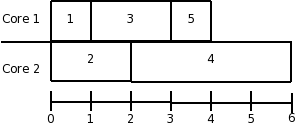
\includegraphics[height=50px]{../img/nich_so_opt_prozessor_belegung.png}
	\end{figure}
}

\frame{
	\frametitle{Analyse}
	\begin{enumerate}
		\item  Sei $Z_k = s_k + l_k$ die Zeit in der der $k$-te Task endet.
		\item  Sei $T_{last}$ der Task der als letztes beendet wird.
		\item  Dann ist die Gesamtlaufzeit $Z_{gesamt} = s_{last} + l_{last}$
		\item <+->  Damit ist die durchschnittliche Laufzeit bis zum Start des letzten Jobs höchstens: $\frac{1}{n}\sum_{k\in\{1,..,i\} \text{\textbackslash} \{last \}}l_k$
		%summe aller laufzeiten bis ausser dem letzten / anzahl der maschinen
		\item <+-> Es existiert also mindestens ein Prozessor dessen Gesamtlaufzeit \textbf{höchstens} von dieser Größe ist, also:	
		$s_{last} \leq \frac{1}{n}\sum_{k\in\{1,..,i\} \text{\textbackslash} \{last \}}l_k$
	\end{enumerate}
	\note{4. Schubfachschluß!}
}

\frame{
\frametitle{Analyse}
\begin{enumerate}
	\item $s_{last} \leq \frac{1}{n}\sum_{k\in\{1,..,i\} \text{\textbackslash} \{last \}}l_k$
	\item offensichtlich gilt: $OPT \geq l_{last}$ %(Optimum entspricht der Optimalen verarbeitungsdauer)
	\item ebenso: $OPT \geq \frac{1}{n}\sum_{k = 1}^{i} l_k$
\end{enumerate}
\note{auch hier ist bei 3. Schubfachschluss}
}

\frame{
\frametitle{Analyse}

\begin{align}
	Z_{gesamt} &= Z_{last} \\
	&= s_{last} + l_{last} \\
	&\leq \frac{1}{n}\sum_{k\in\{1,..,i\} \text{\textbackslash} \{last \}}l_k + l_{last} \\
	& = \frac{1}{n}\sum_{k = 1}^{i} l_k + \left(1-\frac{1}{n}\right) l_{last}\\
	&\leq OPT + \left(1-\frac{1}{n}\right) * OPT \\
	& = \left(2-\frac{1}{n}\right)*OPT
\end{align}
}
\subsection{Ergebnis}
\frame{
\frametitle{Ergebnis}
\begin{block}{Und jetzt?}
	\begin{itemize}
		\item Wir haben gerade gezeigt das \textsc{List Schedule} eine relative Güte von $\left(2-\frac{1}{n}\right)$ hat. (juhu!)
		\item Kann als Basis genutzt werden um \textsc{List Schedule} zu verbessern
		\begin{itemize}
			\item Eingabe komplett erfassen und Sortieren
			\item Alternativ nur vorhandene Eingabe sortieren und den rest nach altem Verfahren sortieren usw.
		\end{itemize} 
	\end{itemize}
\end{block}
}

\section{Fragen}
\frame{
\frametitle{Fragen?}
\begin{center}
	Fragen?
\end{center}
}

\frame{
\frametitle{Ende}
\begin{block}{Quellen}
	Diese Präsentation beruht auf der Ausarbeitung im Rahmen dieses Fachseminars. Sämtliche Quellen sind dort zu finden.
\end{block}
}
\end{document}
